\documentclass[runningheads,a4paper]{llncs}

\usepackage[english]{babel}
\usepackage[utf8]{inputenc}
\usepackage{amsmath}
\usepackage{graphicx}
\usepackage[colorinlistoftodos]{todonotes}
\usepackage{physics}
\usepackage{hyperref}

%\DeclareMathOperator{\Tr}{Tr}

\title{Multi Robots as Delocalized Dexterous Manipulator: a Case Study in Out-of-Plane Rolling via Simple Pushing Robots}

\author{David L. McPherson \and Ronald S. Fearing}

\institute{Biomimetic Millisystems Lab \\
University of California Berkeley \\
Department of Electrical Engineering and Computer Science
}

\date{\today}

\begin{document}
\maketitle

\section{Motivation, Problem Statement, Related Work}

As robots make the migratory leap from well-controlled factory cages into the rough-and-tumble of natural environments, a growing theme is physical interaction.
Locomotive physical interactions are necessarily becoming more complex as the robot is tasked with facing more draconian domains and steeper terrains.
Sticky crawlers, hexapods, snakes, tumbling robots, whegs, wheel robots, MIT cheetahs, bipedal walkers: all these locomotion types require more finesse in the physical interaction between the robot and its terrain.
Here physical interactions are between the robot and its surrounding terrain.
The object being "manipulated" is the robot's body as its position evolves through the space.

More complex physical interactions are also being pioneered in the realm of grasping and manipulation.
The science of grasping kinematics and dynamics were refined for factory pick-and-place robots with high precision, high gain controllers moving steely fingers precisely to stiff locations.
However, as robots leave the factory, they no longer have the luxurys previously assumed by past developments.
Robots no longer know the exact initial position of target parts.
Indeed, the target part may be unstably tumbling about in unknown ways.
To remedy this misfortune, ingenious engineers are working towards compliant grapsing that naturally includes more forgiveness in the mechanics (see Bicchi et. al \cite{BicchiCompliant}).
Pioneers have even delved into manipulation frameworks that preclude the need for static force or form closure.
These frameworks (such as dynamic manipulation (Mason et. al \cite{Lynch01011999}) and dexterous manipulation (Fearing et. al \cite{fearing1986simplified})) allow for more robust manipulations by leaving certain freedoms unconstrained and moving the object within these freedoms.
This all builds on and improves the solutions already obtained for factory grasps and manipulation, leveraging our rich past in engineering grasping to build more robust techinques for the tumultuous environs of tomorrow's robots.
Here the physical interactions are between a robot hand and a target object to be manipulated.

In this work we seek to fuse these two realms of physical interaction and perform manipulation via locomotion.
Objects in the robots environment can be manipulated by pushing.
The core of our proposition here is to use this pushing coupled with effector design and coordinated pushing maneuvers to achieve 5DOF manipulation of objects in the environment.
Rus et al.\cite{rus1995moving} demonstrated techniques for coordinating robots to manipulate furniture in the plane with 3DOF (x,y,yaw).
Sugar et al. \cite{sugar2002control} followed up by digging deeper into the controls for such a team of robots manipulating objects in the plane.
This research extends the capabilities of a team of robot manipulators moving in the plane to enable manipulating objects to roll out of the plane.
We can achieve this without adding grippers or claws or other additional actuators.
Instead, we design the shape of the robot so that the pushing contact surface will roll the target object out of plane.

We take the first step in this brave new world with a case study in manipulating one particular type of object: a capsized robot in the same heterogeneous team as our manipulators.
This case study makes for an exciting motivating application by allowing the heterogenous swarm to self-correct.
Simultaneously, insights into why the general problem is difficult can be glimpsed through the lens of this initial case study.
Finally, the capsized robot's shape (half an ellipsoid) is a fair surrogate for a class of convex polyhedra.

\clearpage
\section{Technical Approach}
\subsection{Robotic Platforms}
The Biomimetic Milllisystems Lab at Berkeley has been investigating group exploration using a heterogenous team of two types of robots.
The first robot is the lightweight and highly mobile RoACH robot \cite{RoACH}.
This robot is modeled after the American Cockroach due to its wide variety of high speed, stable gaits.
However, this robot is also prone to landing inverted on its back and being incapable of righting.
Previous work has investigated additional actuators and mechanisms for getting the robot back on its feet.
However, we are interested in keeping the number of actuators low, for the sake of an affordable robot swarm.
We can achieve the same righting behavior by simply tuning some team member's shape for out-of-plane rolling.

The second robot The platform is codenamed "Zumy" and is shown in Fig. 1.
A further description of the experimental system can be found at \url{https://wiki.eecs.berkeley.edu/biomimetics/Main/Zumy}.
The Zumy platform combines a high power ODROID processor with the commercially available Zumo chassis (from Pololu).
The processor can run Linux, ROS, and computer vision algorithms for experiments in sensor fusion, SLAM, and swarm control.
This work will not leverage the strength of the ODROID processor for much.
Instead, the capable tank-tread design provides a steady locomotion base for transporting around the real focus of this study: a carefully shaped plow.
Two 1600mA, 6V, 30 oz-in miniature motors differentially drive the robot's treads and provide sufficient push force behind our plow.

\subsection{Effector Design}

Here we extend the rich history of research in manipulation to when the "robot hand" is not one connected mechanism, but instead a disconnected team of independent robots.
Distances between the individual fingers are not tightly constrained as in a traditional dexterous hand where all fingers are linked to a unifying palm.
However, our robots have the added constraint of being grounded to move in the plane rather than flex through three dimensions like traditional fingers.

To overcome this shortcoming, we do not design the fingers to rigidly enclose the object (force or form closure) and secure the object in a grasp as in a traditional pick-and-place schema.
Defaulting to a pick-and-place schema is not available to our robots, since the "hand" cannot freely move everywhere (as is assumed in pick-and-place).
Instead the robots are constrained to operate in the plane. Stuck to the ground and unable to fly.
This constraint means in a pick and place schema, the object can be manipulated through as many dimensions as the robot \"hand\" does.
Here our robots only have three DOF on the plane (x,y,yaw).
We will still use the pick-and-place schema for achieving manipulations in these three DOF, but if we want full manipulation (including: roll, pitch, and z) we need something more for our manipulation.

Enter the tumbling manipulation mode -- and the required shape-for-contact design requisite to it.
By abandoning the notion of a closure-sealed grasp, our robot can leverage carefully controlled slippage through dexterous manipulation to achieve extra DOF.
We will build on work by \cite{fearing1986simplified}, and use a cylindrical contact surface.
This choice for contact surface is well motivated by the cylinder's inherent instability in contact.
This instability will tend to push any contacted object up and over the cylinder, allowing exciting new modes for manipulation (as we will see shortly).
The cylindrical contact surface on the front of the robot, is paired with a backstop contact surface on the back of the robot.
Our robots can choose to engage an object with either of its two faces (front plow or backstop).
The backstop surface can fix the object at a point and form a hinge.
This hinge can then be leveraged by another robot pushing the object. Teamwork!

\subsection{Previous Work}
In their seminal paper,
Rather than add an active flipping arm or mechanism, we will use purely passive kinematics of the pushing robot's shape to manipulate the object.
Shape designs for reorienting objects have been thoroughly explored in the robot hand literature.
Rodriguez et al.\cite{rodriguez2013effector} derived the desired shape for an end effector given a target motion.
Zhang et al.\cite{zhang2002gripper} investigated how parallel jaws can reorient objects vertically.
Fearing et al. \cite{fearing1986simplified} used cylindrical fingers to allow objects to roll to a new equilibrium.
This work will similarly investigate how designing just the contact shape can result in desired manipulations.

\clearpage
\section{Results}
Recall that each robot is designed with a pushing surface on the front and a hinging surface on its back.
The robot can choose to engage an object with either of these surfaces since it moves with unicycle kinematics.
We considered two types of front pushing surfaces: plow and cylindrical roller (see Fig. \ref{fig:psurfaces}).
We also considered two types of hinging surfaces: frictive wall and entrapping hinge (see Fig. \ref{fig:surfacesh}).

\begin{figure}[h!]
\centering
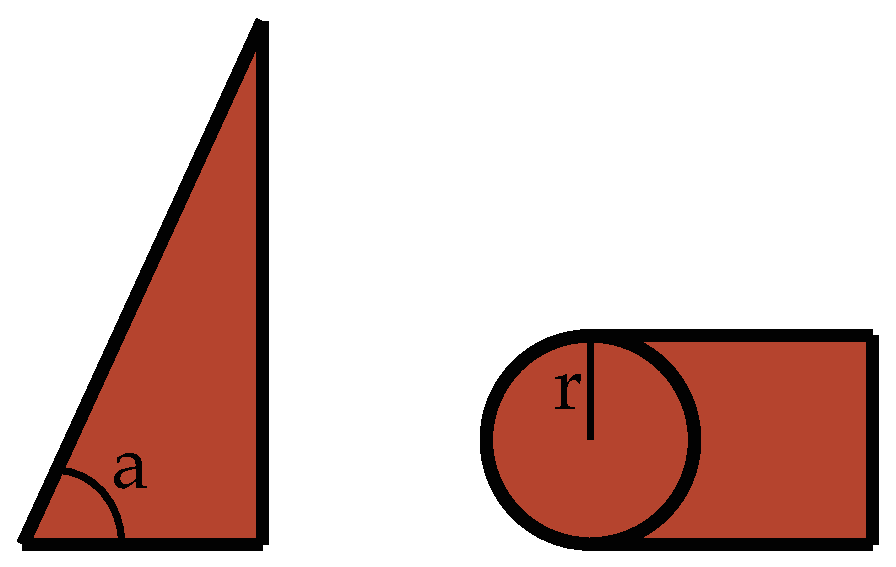
\includegraphics[width=0.3\textwidth]{PlowSurfaceTypes.eps}
\caption{\label{fig:psurfaces}Pushing Surface Types: (left) plow (right) roller}
\end{figure}

\begin{figure}[h!]
\centering
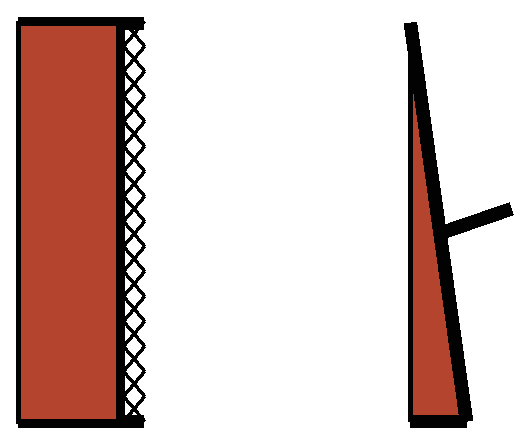
\includegraphics[width=0.3\textwidth]{HingeSurfaceTypes.eps}
\caption{\label{fig:surfacesh}Hinge Surface Types: (left) friction plane (right) entrapping hinge}
\end{figure}

We investigate how these designs can flip a semi-ellipsoidal object as stand-in for general target polyhedra.
We believe the ellipsoid is a fair indicator of flipping ability since it is a polyhedron taken to the limit with infinite sides.
Ellipsoids are used emblematically in the grasping literature as well since they are among the most difficult to grasp due their inherent instability.

To gain insight into how these designs would flip, we plot the trajectories that the ellipsoid will roll through as the plow finger and hinge finger approach each other.
We use kinematics to determine the ellipsoid's configuratin dependent on plow position and then calculate the friction and normal forces quasi-statically.
We highlight the sections of the traces where a frictive surface will act as a perfect hinge using friction force.

\begin{figure}[h!]
\centering
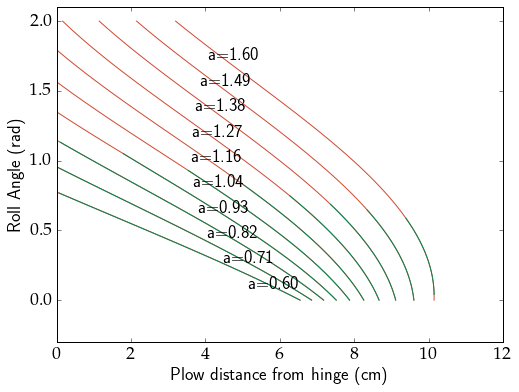
\includegraphics[width=0.3\textwidth]{PlowFlipTrace.png}
\caption{\label{fig:plow}Trace of object roll w.r.t plow distance from hinge}
\end{figure}

\begin{figure}[h!]
\centering
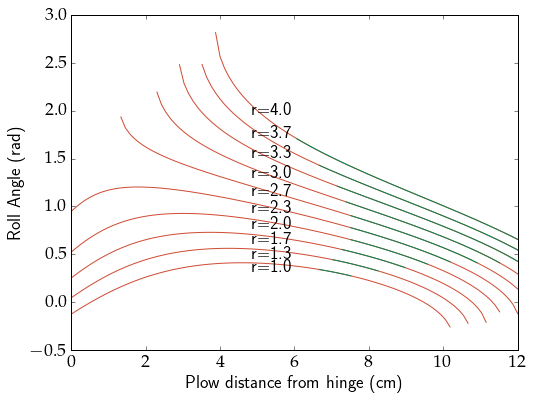
\includegraphics[width=0.3\textwidth]{RollerFlipTrace.png}
\caption{\label{fig:roller}Trace of object roll w.r.t roller distance from hinge}
\end{figure}

We then tested the cylindrical pushing surface paired with an entrapping hinge.
The experiments positively confirmed that this setup can roll the ellipsoid.
Our robot "fingers" can manipulate objects out of the plane with roll successfully!

See Fig. \ref{fig:photos}

\begin{figure}[h!]
\centering
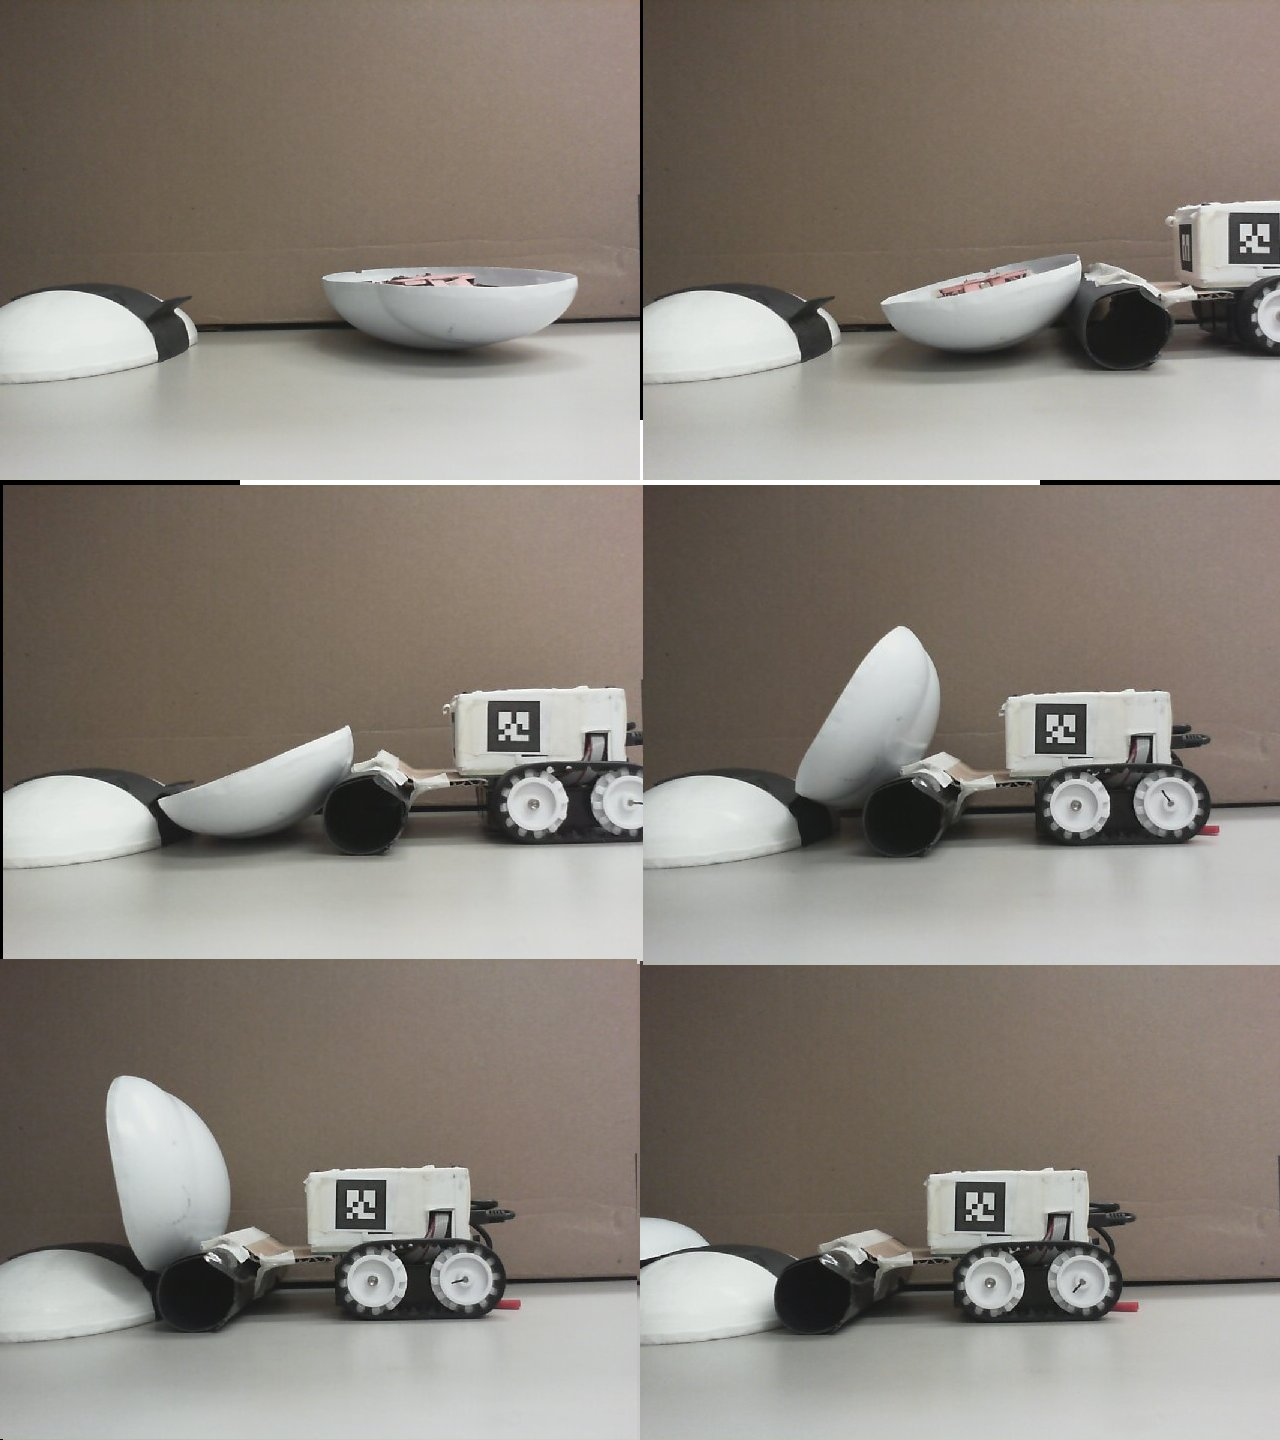
\includegraphics[width=0.3\textwidth]{Photo_Sequence.jpg}
\caption{\label{fig:photos}Photo Sequence of Experimental Flipping}
\end{figure}

\clearpage
\section{Scheduled Experiments}
Scheduled experiments will quantify the breadth of objects that combining finger shape design and treating robots as a delocalized hand's fingers can successfully handle.
We will use the system communication architecture illustrated in Fig. \ref{fig:system}.
This architecture will allow coordinated control of a team of robot fingers to enact trajectories to manipulate a target object.

\begin{figure}[h!]
\centering
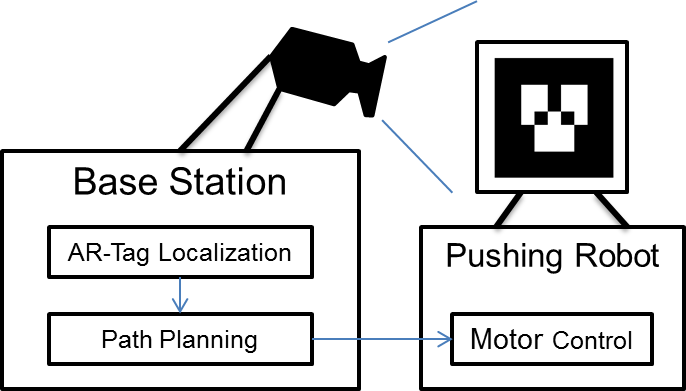
\includegraphics[width=0.3\textwidth]{System_Block_Diagram.png}
\caption{\label{fig:system}Information Flow and Block Diagram of Robot System}
\end{figure}

We will experiment on the flipping characteristics for more target shapes such as classic polyhedra and semi-cylinders.
We also wish to extend our manipulation to the analogue of compliant grasps, when the mass of the object and the fingers are in the same order of magnitude.
In this scenario, the fingers are no longer certain to move to the desired position, but instead will be pushed back by the target object compliantly.
This would allow us to have the finger robots manipulate a fellow robot in their swarm as the target object opening up avenues for complex cooperative maneuvers leveraging this manipulation.

\clearpage
\section{Main Experimental Insights}
Robots can be used to perform full DOF manipulations of environmental objects using only passive kinematics through shape design.
Analysis for designing robot interface shape for contact can leverage rich, general manipulation theory and translate to new domain of locomotive manipulation.
This allows a swarm to manipulate objects without the need to drive up system complexity and adding extra motors to create gripper systems or articulated plows.
In turn this newly afforded object manipulation capability affords robots a wide array of scintillating new application vistas.
A bevy of bots could clear rubble or other obstacles out of their path to ease transport.
Working together, a supporting squad of bots could hoist up a compatriot into a chimney climbing configuration or push them through a hard-to-reach hole.
Teams of bots could manipulate objects into steps or ramps to allow access to previously inaccessible regions.

% =========== References =========== %
\clearpage
\bibliographystyle{plain}
\bibliography{david}

\end{document}
